\documentclass[10pt,letterpaper]{article}
\usepackage[top=1in,left=1in, right=1in, bottom=1in]{geometry}

% use Unicode characters - try changing the option if you run into troubles with special characters (e.g. umlauts)
\usepackage[utf8]{inputenc}

% biblio
\usepackage[natbib, 
  style=numeric,
  giveninits=true,
  maxnames=1,
  maxbibnames=99,
  doi=false,
  url=false,
  sorting=none]{biblatex}

\addbibresource{library.bib}

%suppress In:
\renewbibmacro{in:}{%
  \ifboolexpr{%
     test {\ifentrytype{article}}%
     or
     test {\ifentrytype{inproceedings}}%
  }{}{\printtext{\bibstring{in}\intitlepunct}}%
}

% line numbers
\usepackage[left]{lineno}

% improves typesetting in LaTeX
\usepackage{microtype}
\DisableLigatures[f]{encoding = *, family = *}

% text layout - change as needed
\raggedright
\setlength{\parindent}{0.5cm}
\textwidth 6in 
\textheight 8.75in


% double line spacing
\usepackage{setspace} 
\doublespacing

% adjust caption style
\usepackage[aboveskip=1pt,labelfont=bf,labelsep=period,singlelinecheck=off]{caption}

% headrule, footrule and page numbers
\usepackage{lastpage,fancyhdr,graphicx}

\renewcommand{\footrule}{\hrule height 2pt \vspace{2mm}}
\fancyheadoffset[L]{2.25in}
\fancyfootoffset[L]{2.25in}



\usepackage{enumitem}

\title{PNAS GPP}
% document begins here
\begin{document}
\vspace*{0.35in}

% title goes here:
\begin{flushleft}
{\Large
\textbf\newline{An ecologically based approach to terrestrial primary production}
}
\newline
% authors go here:

Grayson Badgley\textsuperscript{1,2,+,*},
Leander D.L. Anderegg\textsuperscript{1,3,+},
Joseph A. Berry\textsuperscript{1},
Christopher B. Field\textsuperscript{2,4}
\\ % newline after authors

\bigskip
\small
\begin{enumerate}[itemsep=-1mm]
\item Department of Global Ecology, Carnegie Institution for Science, Stanford, CA, 94305
\item Department of Earth System Science, Stanford University, Stanford, CA, 94305
\item Department of Integrative Biology, University of California, Berkeley, CA, 94720
\item Woods Institute for the Environment, Stanford University, Stanford, CA, 94305
\end{enumerate}
\bigskip
* badgley@stanford.edu\\
+ These authors contributed equally
\end{flushleft}
\normalsize
\linenumbers
\section*{Abstract}
Terrestrial gross primary production (GPP) is both the largest and most uncertain flux within the global carbon cycle. Much of this uncertainty results from the fact that GPP is onerous to measure and is only reliably monitored at roughly 100 canopy-scale sites scattered across the globe. Sparsity of consistent GPP observations at the site-level translates into significant uncertainties in our understanding of the magnitude and spatial distribution of GPP at the global scale. We present a new, ecologically based approach for estimating GPP that takes advantage of the tendency for plants to capture only the amount of sunlight they are capable of efficiently using. Our approach uses a new remote sensing product that is sensitive to both the amount of light captured by plants and the efficiency with which plants use light for photosynthesis. The product is highly accurate in reproducing site-based GPP estimates, yet allows for simple calculation using data available globally for more than three decades. By precisely measuring the investment plants dedicate toward capturing and using light, we estimate global annual terrestrial photosynthesis to be 147 Pg C y\textsuperscript{-1} (95\% credible interval 131-163 Pg C y\textsuperscript{-1}), which is intermediate between prevailing bottom-up machine learning and process-based GPP estimates and the top-down global constraint on GPP from oxygen isotopes. Furthermore, our approach enables the propagation and exploration of multiple sources of uncertainty in our estimation of GPP, allowing for biological, statistical, and retrieval errors to be examined separately and further improvement in our understanding of global photosynthesis.

\section*{Introduction}
Terrestrial photosynthesis (or gross primary production (GPP)) is responsible for fixing anywhere from 119 to 169 Pg C y\textsuperscript{-1}, making GPP both the largest and most uncertain component of the global carbon cycle \cite{Anav2015}. Carbon fixed by photosynthesis in turn provides the basis for practically all life on land, providing a strong motivation for improving global estimates of GPP. It is especially important to understand how GPP might respond to global environmental change, as minor perturbations in terrestrial productivity have implications for global biodiversity, agriculture, and climate change \cite{rockstrom2009safe, running2012measurable}.

Quantifying terrestrial GPP is a complicated task, requiring precise measurements of the exchange of both energy and CO\textsubscript{2} between the land surface and the atmosphere. In these efforts, eddy covariance measurements of land surface CO\textsubscript{2} exchange have proved invaluable for estimating canopy and ecosystem scale photosynthesis and model validation \cite{Baldocchi2001, baldocchi2008breathing}. Despite their utility, eddy covariance measurements are  limited in both time and space; individual flux sites measure CO\textsubscript{2} fluxes over approximately  1 km\textsuperscript{2} and, in any given year, fewer than 100 sites operate globally, representing less than one millionth of total land area \cite{kumar2016}. Such limitations especially hinder the validation of terrestrial ecosystem models, which operate globally at resolutions much greater than a single kilometer and need to integrate over processes with time constants from a fraction of a second to many years. 

As a result, a host of semi-empirical upscaling approaches have emerged for translating site-level CO\textsubscript{2} fluxes to globally gridded photosynthesis estimates suitable for model benchmarking and development. Though many upscaling schemes exist, two approaches are by far the most widely applied: machine learning \cite{beer2010terrestrial, tramontana2016predicting} and remote sensing \cite{Running2004}. Both approaches leverage \textit{in situ} fluxes to construct models relating site-level abiotic characteristics, plant traits, and meteorology to estimate photosynthesis beyond tower footprints. Upscaling allows for both the investigation of the drivers of global photosynthesis \cite{jung2017compensatory, zhao2010drought} and for more extensive benchmarking of photosynthesis models by expanding the temporal and spatial availability of photosynthesis estimates \cite{Bonan2011, Williams2009}.

Yet any upscaling introduces uncertainties into GPP estimates, stemming both from model formulation and model inputs. Machine learning approaches, for example, provide the best possible constraint on GPP based on available data, but they functionally operate as black boxes. As a result, they make it difficult to diagnose the causes and consequences of uncertainty. Upscaling approaches are also limited by the availability of and the uncertainties contained within input datasets (e.g. meteorological data). Combined, these challenges limit the utility of upscaling for improving our process-based understanding of photosynthesis and determining the true value of global GPP. Presently, there exists a large and persistent disconnect between upscaled estimates of global GPP and higher estimates derived from top-down isotopic constraints~\cite{Welp2011}.

Here, we report a novel approach for estimating global GPP that avoids many of the limitations posed by upscaling. The approach uses the near-infrared reflectance of vegetation (NIR\textsubscript{V}), a reflectance-based index that is highly correlated with measured site-level GPP \cite{Badgley2017}. This correlation is a consequence of NIR\textsubscript{V} integrating information on both canopy light capture and time-averaged light-use efficiency, which does not have a unique spectral signal, but is instead expressed  through canopy structure. Plants endeavor to capture only the light they are capable of using; any strategy capturing more or less light would be inefficient and subject to the pressures of natural selection \cite{Bloom1985}. This optimality criterion, termed the resource balance or co-ordination hypothesis, means any measure of investment in light capture can serve as the basis for estimating GPP \cite{Field1991, Field1995}. Investment in light capture provides an index of canopy potential photosynthetic capacity, which should in turn closely match total resource availability. This approach has a long history in estimating net primary production (NPP) or biomass production, beginning with Monteith, who showed that a number of agricultural crops all converted sunlight into dry matter at a rate of approximately 1.4 g MJ\textsuperscript{-1} \cite{monteith1977}. The light-use efficiency approach was subsequently extended to use satellite-based measures of light capture and applied to the global scale \cite{Potter1993, Field1995}. But limitations in the available satellite indices meant that accurate GPP estimates required additional information on temperature and moisture levels. Because NIR\textsubscript{V} integrates both light capture and light-use efficiency, it provides a uniquely useful index of investment in light capture and should be sufficient for estimating GPP without additional information on meteorological conditions.  This avoids limitations in data availability and makes our approach capable of estimating GPP at high spatial resolution.  

We present our results in three parts. First, we validate the NIR\textsubscript{V}-GPP relationship at the site and global scale. Second, we extend the relationship to consider global GPP. Third, we evaluate some limitations in the global dataset of NIR\textsubscript{V} and in the consistency of the NIR\textsubscript{V}-GPP relationship. 

\section*{Results}
Using Bayesian hierarchical modeling, we found that NIR\textsubscript{V}, combined with information on ecosystem type (deciduous, evergreen, and crop) explained 68\% of the variation in annual GPP at 105 CO\textsubscript{2} monitoring sites (526 site-years that passed quality-control and data completeness requirements) and had an RMSE of 0.36 kg C m\textsuperscript{-2} y\textsuperscript{-1} (Fig. \ref{fig:site_validation}, see Methods). The approach required no additional information on meteorological conditions, such as site temperature or incoming radiation, indicating that NIR\textsubscript{V} captures the effects of meteorology on GPP and supporting our interpretation of NIR\textsubscript{V} as an integrator of whole-plant resource optimization (Fig. S1). Fewer inputs not only reduces uncertainty from input datasets, but also allows the NIR\textsubscript{V} approach to be applied across a wide range of spatial and temporal scales. By contrast, existing remote sensing and machine learning based approaches for estimating GPP often require tens to hundreds of inputs.  The NIR\textsubscript{V} approach performed similarly well at the monthly time scale (Fig. \ref{fig:site_validation}, inset), explaining 56\% of the observed variation in monthly GPP with an RMSE of 0.08 kg C m\textsuperscript{-2} mo\textsuperscript{-1}. The RMSE of NIR\textsubscript{V}-based estimates of annual GPP was 42\% lower than the RMSE of GPP fluxes calculated from BESS, a physiologically based land surface model, and was 57\% higher than GPP estimates from  FLUXCOM, a meteorological-based, statistical upscaling of FLUXNET GPP fluxes (Table S1).  

For annual GPP, the most parsimonious model included just three ecosystem types, with a single intercept and separate NIR\textsubscript{V}-GPP slopes for sites with i) evergreen, ii) deciduous, and iii) crop ecosystem types, as well as increasing variance in both residual error and site-level random intercepts as a function of NIR\textsubscript{V} (Fig. S2). Further dividing ecosystem types resulted in minor model improvements, but an almost identical Deviance Information Criteria with more parameters, causing us to adopt the simpler three ecosystem type model (see Methods). 

\begin{figure}[t]
    \centering
    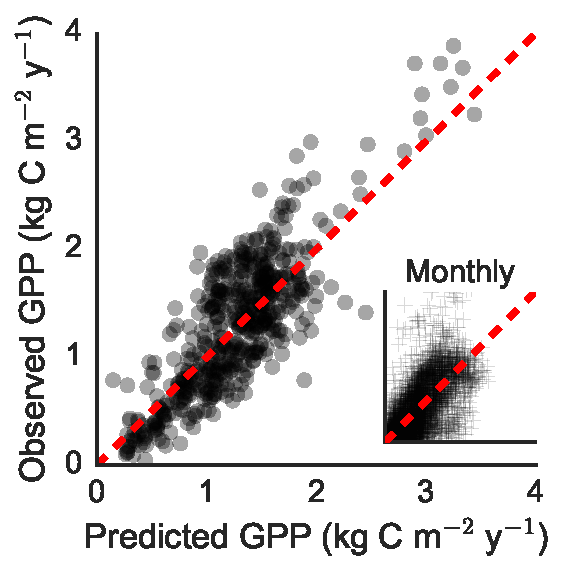
\includegraphics[width=0.4\textwidth, keepaspectratio]{figure_validation_inset.pdf}
    \caption{\textbf{NIR\textsubscript{V} explains a large portion of site-level GPP at both the monthly and annual timescale}. Note the relatively large variation in monthly GPP estimates for low values of observed GPP, as compared to the near-zero intercept in the case of annual fluxes.}
    \label{fig:site_validation}
\end{figure}

Applying this site-level scaling to globally resolved measurements of NIR\textsubscript{V}, we estimated the median value of global annual GPP to be 147 Pg C y\textsuperscript{-1}, with a 95\% credible interval of 131-163 Pg C y\textsuperscript{-1}. Our median GPP estimate is intermediate between estimates from spatial models and constraints from O\textsubscript{2} isotopes. FLUXCOM places annual GPP at 118 Pg C y\textsuperscript{-1}, while BESS puts mean global GPP at 122 Pg C y\textsuperscript{-1}.  A meta-analysis of model-based annual GPP estimates ranged from 119 to 169 Pg C y\textsuperscript{-1} \cite{Anav2015}. By contrast, O\textsubscript{2} isotopic measurements are consistent with global annual GPP in the range of 150 to 175 Pg C y\textsuperscript{-1} \cite{Welp2011}. 

\begin{figure}
    \centering
    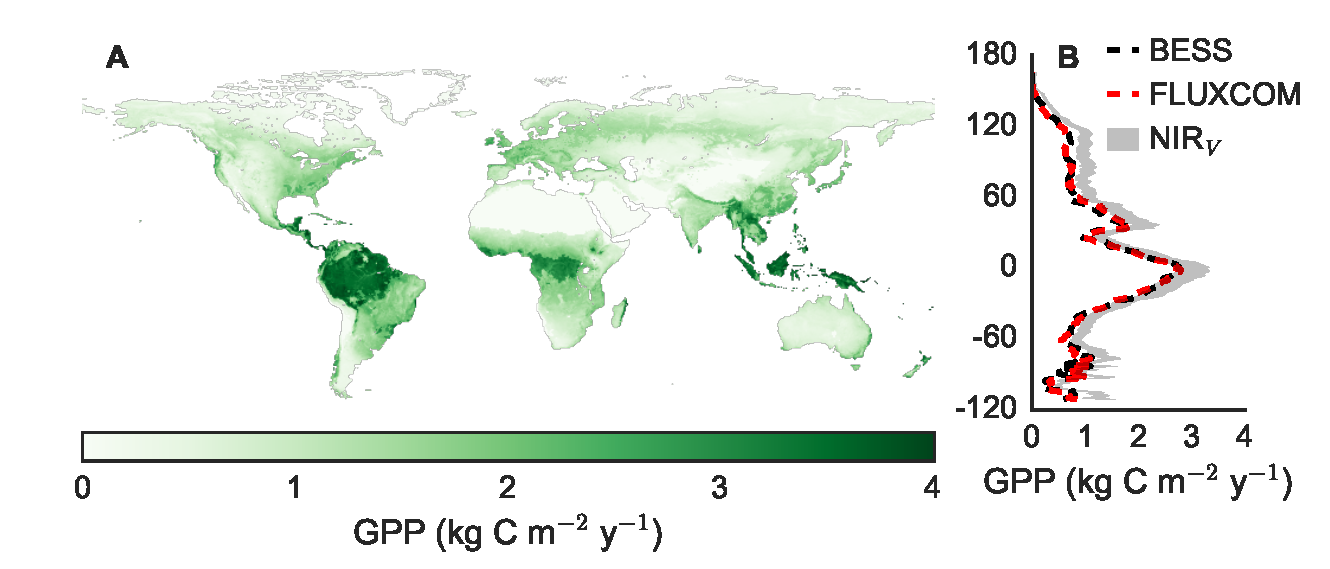
\includegraphics[width=\textwidth, keepaspectratio]{figure_nirv_gpp_map_area.pdf}
    \caption{\textbf{The A) global and B) latitudinal distribution of NIR\textsubscript{V}-derived GPP.}  Estimates represent the median of 1000 nearly independent upscalings of NIR\textsubscript{V}, while the full 95\% credible range of GPP is shaded in grey for latitudinal estimates. The latitudinal distribution of annual GPP from FLUXCOM and BESS are shown for comparison. }
    \label{fig:gpp_map}
\end{figure}

The spatial distribution of NIR\textsubscript{V}-derived GPP was consistent with existing global GPP estimates, further validating our approach  (Fig. \ref{fig:gpp_map}). As expected, GPP was concentrated in the tropics and declined toward the poles. On a per biome basis, tropical forests contributed the most to global GPP, accounting for 31\%  of global GPP; FLUXCOM and BESS attribute 34\% and 33\% of GPP to tropical forests, respectively. Though lower in relative terms, NIR\textsubscript{V}-derived GPP in tropical forests was 15\% higher than both FLUXCOM and BESS GPP estimates in absolute terms.  Instead, NIR\textsubscript{V} assigned higher productivity to the midlatitudes, especially  midlatitude mixed forests, grasslands, and shrub-dominated ecosystems (Fig. \ref{fig:gpp_map}B; Table S2). One recent study that combined solar-induced chlorophyll fluorescence with a terrestrial ecosystem model found similar relative increases in extratropical GPP \cite{Norton2018}.

When compared on a per pixel basis, NIR\textsubscript{V} was strongly linear with both FLUXCOM and BESS at the annual time scale, with R\textsuperscript{2} exceeding 0.90 for both products and per pixel RMSE below 0.4 kg C m\textsuperscript{-2} y\textsuperscript{-1}, further emphasizing the robustness of NIR\textsubscript{V}-derived GPP estimates (Fig. \ref{fig:bess_fluxcom}). This consistency is striking, given that our approach employed only two variables (NIR\textsubscript{V} and ecosystem type), while both FLUXCOM and BESS require numerous environmental inputs. The comparison also emphasizes that NIR\textsubscript{V}-derived GPP estimates are consistently higher than existing approaches, exceeding FLUXCOM GPP by a median value of 0.24 kg C m\textsuperscript{-2} y\textsuperscript{-1} and BESS GPP by 0.21 kg C m\textsuperscript{-2} y\textsuperscript{-1}. There are several possible reasons for this difference. On one hand, NIR\textsubscript{V} might represent a theoretical upper bound of photosynthesis, prior to consideration of physiological effects (e.g.,  water or nutrient limitation), causing NIR\textsubscript{V}-based GPP estimates to outpace physiologically based approaches. Alternatively, both BESS and FLUXCOM might systematically underestimate true GPP. Investigating the source of this discrepancy through more detailed comparisons of NIR\textsubscript{V} against eddy covariance data and site-level modelling represents an important next step in using NIR\textsubscript{V} to study photosynthesis at the global scale.

\begin{figure}
    \centering
    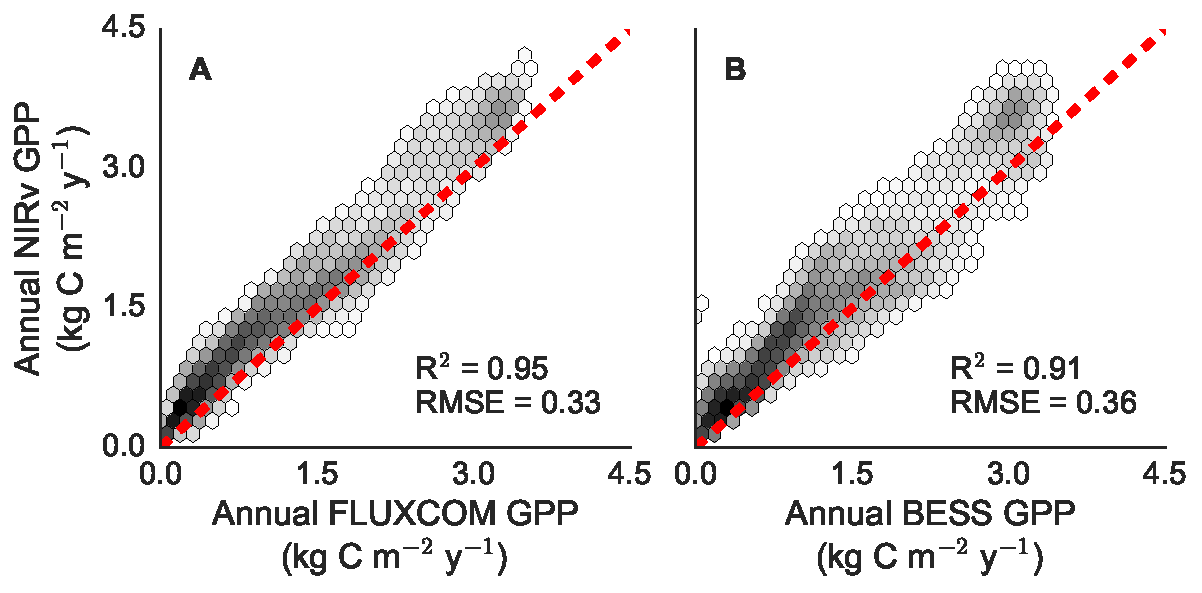
\includegraphics[width=11.4cm, keepaspectratio]{figure_bess_fluxcom_area.pdf}
    \caption{\textbf{Upscaled NIR\textsubscript{V}-based estimates of annual GPP are linear with both A) FLUXCOM and B) BESS GPP estimates}.  NIR\textsubscript{V}-based estimates tend to be slightly higher than both FLUXCOM and BESS, though NIR\textsubscript{V} has low a RMSE relative to both products. NIR\textsubscript{V}-based GPP estimate shown as the median case of 1000 nearly independent upscalings, see Methods. }
    \label{fig:bess_fluxcom}
\end{figure}

Model parsimony, combined with Bayesian estimation, allowed us to propagate three sources of uncertainty on a per pixel basis: statistical, variation in per ecosystem type scaling; site, deviation of a site intercept from the global per ecosystem type relationship; and residual, or otherwise unexplained errors. Median per pixel uncertainty was 0.20 kg C m\textsuperscript{-2} y\textsuperscript{-1} and total uncertainty, comprising all three sources of error, peaked in the tropics where total annual NIR\textsubscript{V} was highest. In the worst case, the 95\% credible interval of GPP exceeded 0.75 kg C m\textsuperscript{-2} y\textsuperscript{-1} in the Amazon basin and Indonesia (Fig. \ref{fig:uncertainty_map}A). Given that tropical forests constitute the highest proportion of GPP (exceeding 30\%), high uncertainty throughout the tropics significantly contributes to the overall uncertainty of global GPP estimates, regardless of approach. 

Informative patterns emerge from examining the relative importance of statistical, site, and residual uncertainty on a per pixel basis; two examples of pixel-level uncertainties are shown in Fig. \ref{fig:uncertainty_map}B. Outside of pixels with especially low NIR\textsubscript{V}, statistical uncertainty was always lowest, indicating minimal uncertainty in per ecosystem type scaling.  On average, site uncertainty was always largest, meaning there was more uncertainty in the NIR\textsubscript{V}-GPP relationship from site to site than existed year to year (encompassed by residual uncertainty) at a single site. This indicates that either NIR\textsubscript{V} or GPP estimates are not comparable across sites, which must be addressed by improving the accuracy of both measurements. The predominance of site-level uncertainty is a direct result of considerable variation in site-level intercepts (Fig. S1). Site-to-site variability is randomly distributed, showing no relationship with site climate, thus highlighting retrieval errors (e.g., soil reflectance, clouds) as the likely cause of site-level uncertainty.

\begin{figure}
    \centering
    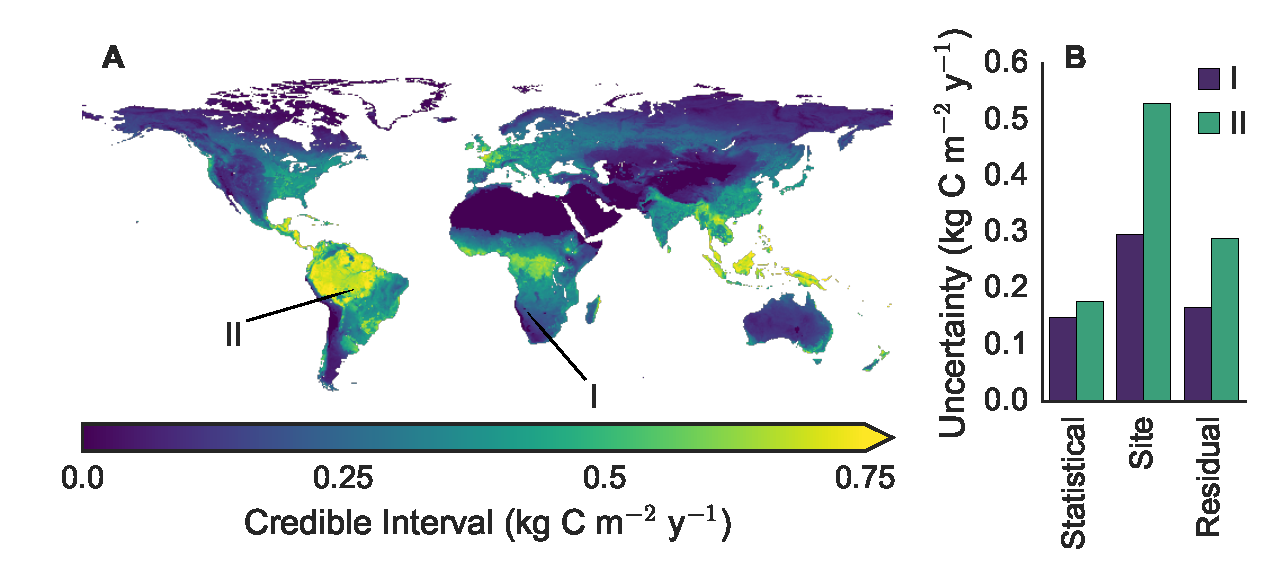
\includegraphics[width=\textwidth, keepaspectratio]{figure_uncertainty_area.pdf}
    \caption{\textbf{Bayesian hierarchical modeling allows for per pixel error estimation}. A) Uncertainty in GPP peaks in the tropics (especially the Amazon and Indonesia), where the credible range of GPP exceed 0.75 kg C m\textsuperscript{-2} y\textsuperscript{-1}. B) Uncertainty can be evaluated on a per pixel basis, where  site-level uncertainty is typically largest.}
    \label{fig:uncertainty_map}
\end{figure}

\section*{Discussion}
NIR\textsubscript{V} takes advantage of a globally consistent relationship between canopy structure and photosynthetic potential to provide  an ecologically grounded approach for estimating GPP that combines a very simple formulation with excellent performance at validation sites (Figs. \ref{fig:site_validation} and \ref{fig:bess_fluxcom}). As a result, NIR\textsubscript{V} provides a novel means for  upscaling GPP flux measurements  that is largely independent of existing and widely used semi-empirical and process-based approaches. Finally, the NIR\textsubscript{V} GPP approach achieves strong statistical performance while maintaining parsimony, allowing for i) an evolutionary and ecologically mechanistic interpretation of upscaling results, ii) straightforward analysis of uncertainty and how uncertainty is partitioned between model structure and inputs (Fig. \ref{fig:uncertainty_map}), and iii) simple calculation.

Parsimony allows for a mechanistic interpretation of the NIR\textsubscript{V}-GPP relationship, in terms of how NIR\textsubscript{V} and GPP jointly relate to canopy architecture and light capture. From a physical standpoint, NIR\textsubscript{V} relates to variations in canopy leaf area and leaf display, serving as a useful index of the investment plants dedicate toward processing the light they capture \cite{Badgley2017}. Consistent with the resource balance hypothesis, plants tend to capture only as much light as they are capable of using \cite{Field1991}, helping explain the strength of the NIR\textsubscript{V}-GPP relationship that otherwise has no strong physiological basis (Fig. \ref{fig:site_validation}). On an instantaneous basis, environmental factors like water, light, and temperature combine with leaf-level biochemical capacity to dictate the rate of photosynthesis; insights that are enshrined in leaf-level photosynthesis models \cite{FvCB}.  The predictive ability of NIR\textsubscript{V}, without the need for additional inputs like total incoming radiation, does not imply that environmental factors are irrelevant to photosynthesis, but rather that canopy architecture represents an emergent property that encapsulates the mechanistic controls of photosynthesis.

This mechanistic interpretation of the NIR\textsubscript{V}-GPP relationship has implications for terrestrial photosynthesis models.  We postulate that neglecting changes in canopy architecture within models can cause decoupling of light capture and canopy physiology. Models typically hold canopy architectural parameters (e.g., the ratio of sun and shade leaves) constant and instead vary leaf physiological parameters, like the maximum rate of carboxylation (V\textsubscript{Cmax}). During periods of peak growth, for example, a model might underestimate light capture and compensate by arbitrarily adjusting V\textsubscript{Cmax} to match GPP observations. This can result in V\textsubscript{Cmax} becoming a model-dependent parameter, as opposed to a biologically interpretable measurement \cite{Bonan2011}. Future studies should consider combining measurements of NIR\textsubscript{V} and V\textsubscript{Cmax} to address this problem. These data would allow for independently fixing model V\textsubscript{Cmax} using empirical data, while simultaneously varying canopy architecture as a function of observed NIR\textsubscript{V}. Such an experiment would capitalize on the empirical NIR\textsubscript{V}-GPP relationship to improve how process-based models represent both light capture and leaf physiology. 

Another strength of the NIR\textsubscript{V} approach is that it allows statistically valid error propagation (Fig. \ref{fig:uncertainty_map}). More complicated approaches to estimating GPP make it difficult to accurately partition sources of error, especially model structural errors and errors due to input uncertainties. Minimizing upscaling complexity largely eliminates this problem. In particular, we were surprised by the predominance of site-level error;  the NIR\textsubscript{V}-GPP relationship always varied more from site to site than within a single site (Fig. \ref{fig:uncertainty_map}B). This indicates that either the biology controlling the NIR\textsubscript{V}-GPP relationship itself  varies from site to site or that NIR\textsubscript{V} and GPP measurements lack consistency across space. More simply, if the NIR\textsubscript{V}-GPP relationship holds in general, deviations from this relationship should have either a biological or a methodological interpretation. The simplicity of our approach allows for the investigation of both possibilities. 

As an example of measurement challenges, there is a stark disagreement in the NIR\textsubscript{V}-GPP relationship at an eddy covariance site in French Guyana, GF-Guy. GPP fluxes at GF-Guy varied less than 20\% month to month, while NIR\textsubscript{V} varied by a factor of three (Fig. \ref{fig:parsimony_pluses}A). Assuming accurate GPP estimates, the divergence suggests errors in NIR\textsubscript{V} observations at the site. We suspected cloud contamination, as remote sensing in the tropics is notoriously plagued by clouds degrading the accuracy of satellite measurements. To investigate this, we used the newly available MAIAC data product, which uses atmospheric modelling to remove aerosols, sub-pixel clouds, and other artifacts from MODIS satellite imagery \cite{lyapustin2011multiangle}. The variability of NIR\textsubscript{V} dramatically reduced with the MAIAC data (Fig. \ref{fig:parsimony_pluses}A). In fact, MAIAC-derived NIR\textsubscript{V} had a smaller dynamic range than observed GPP, strongly indicating cloud contamination of the baseline MODIS dataset both at GF-Guy and, in all likelihood, throughout the tropics. Such contamination likely reduces our median global GPP estimate, making 147 Pg C y\textsuperscript{-1} a conservative estimate of global GPP.  We expect that using MAIAC-derived NIR\textsubscript{V} as the basis for estimating GPP would reduce site-level uncertainty and improve the accuracy of global GPP estimates. Unfortunately, such efforts will have to wait for a globally consistent MAIAC reprocessing of the full MODIS record.

\begin{figure}[h]
    \centering
    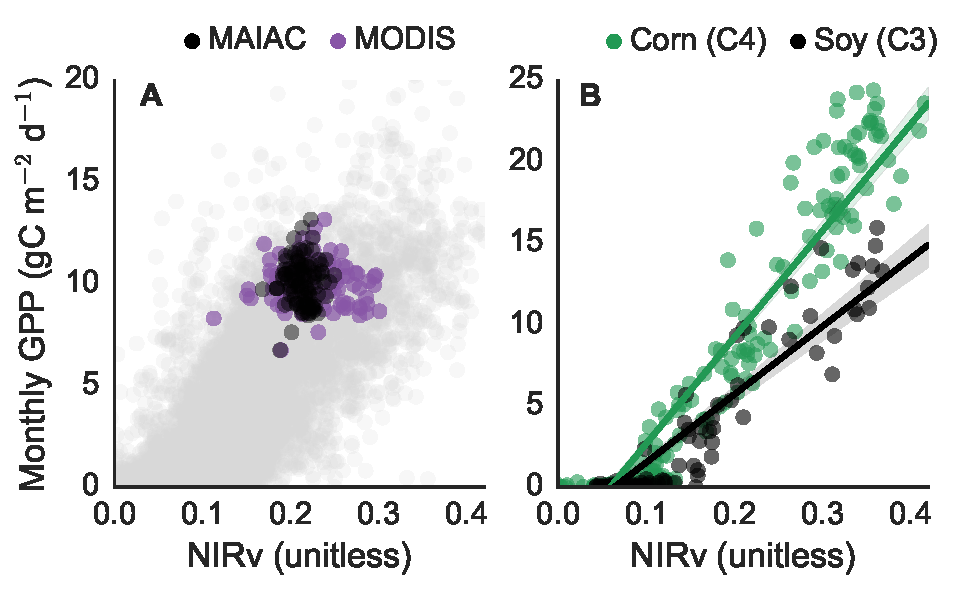
\includegraphics[width=11.4cm, keepaspectratio]{figure_parsimony.pdf}
    \caption{\textbf{Parsimony allows for the investigation of sources of model uncertainty}. A) Cloud contamination drives large monthly variations in MODIS collection 6 NIR\textsubscript{V} that are not matched by variations in NIR\textsubscript{V}. All monthly data from the FLUXNET2015 dataset shown in grey. B) Photosynthetic pathway predictably alters the NIR\textsubscript{V}-GPP relationship, as C4 plants have greater efficiency.}
    \label{fig:parsimony_pluses}
\end{figure}

Fundamental differences in plant physiology that govern the NIR\textsubscript{V} and GPP relationship can also explain the predominance of site uncertainty. In this case, the simplicity of our approach leaves out potentially important biological determinants of productivity. Take for example the difference in C3 and C4 photosynthesis. C4 plants fix CO\textsubscript{2} more efficiently than C3 plants, which should cause a steeper slope in the NIR\textsubscript{V}-GPP relationship, all else equal. When we examined a trio of Nebraskan eddy covariance towers that annually rotate between soy (C3) and corn (C4) crops, we found significant differences in the NIR\textsubscript{V}-GPP slope with crop type (Fig. \ref{fig:parsimony_pluses}B). As with cloud contamination, including information on the distribution of C3 and C4 vegetation across both wild and managed ecosystems would likely increase our global estimate of GPP, as C3 sites comprise the majority of data within the dataset used for calibration. This result further emphasizes the conservative nature of our 147 Pg C y\textsuperscript{-1} estimate of GPP. Apart from indicating that NIR\textsubscript{V}-based GPP estimates could be further improved by incorporating a photosynthetic pathway parameter, this result also demonstrates how our ecologically grounded approach can be used to study plant physiology at the global scale.

The third advantage of the NIR\textsubscript{V} approach is that NIR\textsubscript{V} can be calculated from existing high-resolution and widely available satellite imagery. This makes NIR\textsubscript{V} immediately available for benchmarking models at spatial and temporal scales relevant to land surface models, whether the model runs at 30 meters for a specific study site or spans the globe (Figs. \ref{fig:site_validation} and \ref{fig:bess_fluxcom}). Our approach for estimating GPP from NIR\textsubscript{V} could also be calculated for the full Landsat and MODIS records, as well as the 39 year record of the Advanced Very High Resolution Radiometer (AVHRR) series of sensors \cite{Tucker2005}.  Long-term records that cover a range of climatic conditions are vital for benchmarking physiological models we hope to use in forecasting future ecological change. Finally, the ease of measuring NIR\textsubscript{V} allows researchers to make inexpensive, canopy-scale spectral measurements that are directly comparable against satellite data, facilitating efforts to bridge spatial scales.

To conclude, we have developed a new, largely independent approach for estimating GPP that closely corresponds to existing best-in-class GPP estimates. Our robust handling of uncertainty demonstrates that current estimates of global GPP are likely too low and that the annual productivity of terrestrial ecosystems likely exceeds 147 Pg C y\textsuperscript{-1}, which more closely agrees with top-down, isotopically constrained estimates of GPP \cite{Welp2011}.  Further refinement of our NIR\textsubscript{V}-based approach, through reducing input uncertainty and inclusion of additional physiological processes, will serve as a powerful new tool for validating terrestrial ecosystem models and improving our mechanistic understanding of the terrestrial carbon cycle.   

\section*{Materials and Methods}
\subsection*{Data} We compared NIR\textsubscript{V} against monthly and annual GPP fluxes at 105 flux sites contained in the FLUXNET2015  Tier 1 dataset. For each site, we downloaded 500 meter, daily red (620-670nm) and near-infrared (NIR, 841-876nm) nadir-adjusted reflectances from MODIS collection MCD43A4.006  hosted on Google Earth Engine \cite{MODISv6}. We calculated median NDVI and NIR for all scenes overlapping a 1km\textsuperscript{2} circle around each fluxsite. Gaps were filled using linear interpolation. Finally, we multiplied median NDVI by NIR to calculate NIR\textsubscript{V} and took the average of all daily NIR\textsubscript{V} values for each month. We then combined monthly NIR\textsubscript{V} estimates with monthly observations of GPP from the FLUXNET2015 dataset (variable name: GPP\_VUT\_MEAN). We required all site-months to have over 75\% valid GPP observations and required site-years to have a minimum of 9 months of data. We gridded the MCD43A4.006 dataset to 0.5\textsuperscript{$\circ$} to serve as the basis of our global upscaling.

In addition to the site-level comparisons, we evaluated NIR\textsubscript{V}-based GPP estimates against two existing models of GPP: FLUXCOM, a machine learning approach for upscaling FLUXNET observations \cite{tramontana2016predicting}, and GPP estimates derived from the physiologically based land surface  model, the Breathing Earth System Simulator (BESS), which has been extensively benchmarked against eddy covariance measurements of GPP \cite{ryu2011, jiang2016multi}. We used the mean ensemble of annual GPP\_HB fluxes from the FLUXCOM CRUNCEPv6 product, accessed via the FLUXCOM website. For BESS, we used GPP estimates from BESS V1, obtained from the BESS website. Site-level RMSE values for FLUXCOM and BESS were derived from data provided by the authors \cite{tramontana2016predicting, jiang2016multi}.

\subsection*{Calibration}
We used Bayesian estimation to relate NIR\textsubscript{V} and ecosystem type to GPP at both monthly and annual timescales. Bayesian estimation allows the propagation of uncertainty through hierarchical modeling, which allowed us to fit slope and intercept terms, as well as hierarchical variance terms capturing site-level random effects (random deviations from the global slope and intercept per site) and error variance \cite{Gelman1995}. We specified GPP as a linear function of NIR\textsubscript{V}, with the best model (according to the Deviance Information Criteria; \citep{Gelman1995}) consisting of a single, near-zero intercept and differing slopes for evergreen, deciduous, and crop ecosystem types.  The model included two additional terms: a random site-level intercept term and an error term that were both normally distributed with mean of 0 and variance exponentially related to NIR\textsubscript{V}. See Supplementary Text 1 and Table S3 for a full description of the model structure, as well as alternative model structures tested. 
We used Markov chain Monte Carlo simulations (MCMC) implemented in JAGS \cite{JAGS} to sample the joint posterior distribution of fitted models, with initial diffuse priors for all parameters. We ran three parallel MCMC chains, evaluated chains for convergence, and thinned chains to remove within-chain autocorrelation, producing 1000 nearly independent draws from the posterior. We calculated site-level, median estimates of GPP and 95\% credible intervals for model parameters based on the joint posterior distribution of the best model.  We have posted the GPP calibration code to www.github.com/badgley/nirv-global.

\subsection*{Upscaling}
\raggedbottom
We produced global annual estimates of GPP with the best annual NIR\textsubscript{V} model, using all 1000 draws from the joint model posterior to calculate GPP for all land pixels from 2005 to 2015. For each posterior draw, we calculated GPP of every pixel based on the per-biome scaling parameter plus randomly sampled site-level and residual error based on the site and residual variance parameter estimates for that draw. Using the site-level model for our global upscaling captures correlations between parameter estimates (scaling slope and site-level variance estimates were often correlated), resulting in GPP estimates that appropriately represent statistical, site, and residual uncertainty from the full joint posterior distribution of the model. We present the median and 95\% credible intervals from the distribution of the upscaled GPP estimates. We excluded pixels with a landcover classification of ``barren''.

\nolinenumbers

\section*{Acknowledgments}
We thank J. Johnson and Y. Shiga for the many conversations that clarified our thinking, as well as Y. Ryu and M. Whelan, whom reviewed earlier drafts of this work. G. Tramontana and C. Jiang kindly provided site-level GPP fluxes for comparison. B. Peng shared the C3/C4 crop rotation data. Funds from a NASA Earth and Space Science fellowship (G.B.), a NOAA Climate and Global Change fellowship, and NSF Postdoctoral Research Fellowship Grant No. DBI-1711243 (L.D.L.A) supported this research. Any opinions, findings, and conclusions or recommendations expressed in this material are those of the author(s) and do not necessarily reflect the views of the National Science Foundation.  This work used eddy covariance data acquired and shared by the FLUXNET community, including these networks: AmeriFlux, AfriFlux, AsiaFlux, CarboAfrica, CarboEuropeIP, CarboItaly, CarboMont, ChinaFlux, Fluxnet-Canada, GreenGrass, ICOS, KoFlux, LBA, NECC, OzFlux-TERN, TCOS-Siberia, and USCCC. The ERA-Interim reanalysis data are provided by ECMWF and processed by LSCE. The FLUXNET eddy covariance data processing and harmonization was carried out by the European Fluxes Database Cluster, AmeriFlux Management Project, and Fluxdata project of FLUXNET, with the support of CDIAC and ICOS Ecosystem Thematic Center, and the OzFlux, ChinaFlux and AsiaFlux offices.

\printbibliography


\end{document}